	%%%%%%%%%%%%%%%%%%%%%%%%%%%%%%%%%%%%%%%%%
%           Fichier maitre				%
%%%%%%%%%%%%%%%%%%%%%%%%%%%%%%%%%%%%%%%%%

\documentclass[a4paper, 12pt, twoside,openright]{report}

%%%%%%%%%%%%%%%%%%%%%%%%%%%%%%%%%%%%%%%%
%           Liste des packages         %
%%%%%%%%%%%%%%%%%%%%%%%%%%%%%%%%%%%%%%%%
%%%%%%%%%%%%%%%%%%%%%%%%%%%%%%%%%%%%%%%%%%%%%%%%%%%%%%%%%%%%%%%%%%%%%
\usepackage{tikz}
\usepackage{pgfplots}
%% Réglage des fontes et typo    
\usepackage[utf8]{inputenc}		% LaTeX, comprend les accents !
\usepackage[T1]{fontenc}
\usepackage{natbib}		% Doit être chargé avant babel
\setcitestyle{authoryear,open={[},close={]}}\usepackage{chapterbib}
%	\renewcommand{\bibsection}{\chapter*{Références Bibliographies}}		% Met les références biblio dan
%s un \section (au lieu de \section*)
 
\usepackage[english,frenchb]{babel}
\usepackage{lmodern}
\usepackage{ae,aecompl}	
\usepackage{multicol}									% Utilisation des fontes vectorielles modernes
\usepackage[upright]{fourier}
\usepackage{lipsum}
\usepackage{wrapfig}
%%%%%%%%%%%%%%%%%%%%%%%%%%%%%%%%%%%%%%%%%%%%%%%%%%%%%%%%%%%%%%%%%%%%%
% Allure générale du document
\usepackage{enumerate}
\usepackage{enumitem}
%\usepackage[section]{placeins}	% Place un FloatBarrier à chaque nouvelle section
\usepackage{epigraph}
\usepackage[font={small}]{caption}
\usepackage[francais,nohints]{minitoc}		% Mini table des matières, en français
	\setcounter{minitocdepth}{2}	% Mini-toc détaillées (sections/sous-sections)
\usepackage[notbib]{tocbibind}		% Ajoute les Tables	des Matières/Figures/Tableaux à la table des matières
%%%%%%%%%%%%%%%%%%%%%%%%%%%%%%%%%%%%%%%%%%%%%%%%%%%%%%%%%%%%%%%%%%%%%
%% Maths                         
\usepackage{amsmath}			% Permet de taper des formules mathématiques
\usepackage{amssymb}			% Permet d'utiliser des symboles mathématiques
\usepackage{mathrsfs}
\usepackage{amsfonts}			% Permet d'utiliser des polices mathématiques
\usepackage{nicefrac}			% Fractions 'inline'
\usepackage{nccmath}
%%%%%%%%%%%%%%%%%%%%%%%%%%%%%%%%%%%%%%%%%%%%%%%%%%%%%%%%%%%%%%%%%%%%%
%% Tableaux
\usepackage{multirow}
\usepackage{booktabs}
\usepackage{colortbl}
\usepackage{tabularx}
\usepackage{multirow}
\usepackage{threeparttable}
\usepackage{etoolbox}
	\appto\TPTnoteSettings{\footnotesize}
\addto\captionsfrench{\def\tablename{{\textsc{Tableau}}}}	% Renome 'table' en 'tableau'
%%%%%%%%%%%%%%%%%%%%%%%%%%%%%%%%%%%%%%%%%%%%%%%%%%%%%%%%%%%%%%%%%%%%%
%% Eléments graphiques                    
\usepackage{graphicx}			% Permet l'inclusion d'images
\usepackage{subcaption}
\usepackage{pdfpages}
\usepackage{rotating}
\usepackage{pgfplots}
	\usepgfplotslibrary{groupplots}
\usepackage{tikz}
	\usetikzlibrary{backgrounds,automata}
	\pgfplotsset{width=7cm,compat=1.3}
	\tikzset{every picture/.style={execute at begin picture={
   		\shorthandoff{:;!?};}
	}}
	\pgfplotsset{every linear axis/.append style={
		/pgf/number format/.cd,
		use comma,
		1000 sep={\,},
	}}
\usepackage{eso-pic}
\usepackage{import}
%%%%%%%%%%%%%%%%%%%%%%%%%%%%%%%%%%%%%%%%%%%%%%%%%%%%%%%%%%%%%%%%%%%%%
%% Mise en forme du texte        
\usepackage{xspace}
\usepackage[load-configurations = abbreviations]{siunitx}
	\DeclareSIUnit{\MPa}{\mega\pascal}
	\DeclareSIUnit{\micron}{\micro\meter}
	\DeclareSIUnit{\tr}{tr}
	\DeclareSIPostPower\totheM{m}
	\sisetup{
	locale = FR,
	  inter-unit-separator=$\cdot$,
	  range-phrase=~\`{a}~,     	% Utilise le tiret court pour dire "de... à"
	  range-units=single,  		% Cache l'unité sur la première borne
	  }
\usepackage[version=3]{mhchem}	% Equations chimiques
\usepackage{textcomp}
\usepackage{array}
\usepackage{hyphenat}
%%%%%%%%%%%%%%%%%%%%%%%%%%%%%%%%%%%%%%%%%%%%%%%%%%%%%%%%%%%%%%%%%%%%%
%% Navigation dans le document
\usepackage[pdftex,pdfborder={0 0 0},
			colorlinks=true,
			linkcolor=blue,
			citecolor=red,
			pagebackref=true,
			]{hyperref}	% Créera automatiquement les liens internes au PDF
					% Doit être chargé en dernier (Sauf exceptions ci-dessous)
%%%%%%%%%%%%%%%%%%%%%%%%%%%%%%%%%%%%%%%%%%%%%%%%%%%%%%%%%%%%%%%%%%%%%
%% Packages qui doivent être chargés APRES hyperref	             
\usepackage[top=0cm, bottom=-0.5cm, left=0cm, right=0cm]{geometry}
\usepackage{fancyhdr}
\addtolength{\headheight}{2.5pt}
\fancyhf{}
%\fancyhead[LE,RO]{\nouppercase{\thepage}}
%\fancyhead[L]{\nouppercase{\leftmark}}
\renewcommand{\headrulewidth}{2pt}
\renewcommand{\footrulewidth}{1pt}
\pagestyle{fancy}
\lhead{\nouppercase{\leftmark}}
\rfoot{page \centering \thepage}
\pagestyle{fancy}
\usepackage{tcolorbox}
\usepackage[acronym,xindy,toc,numberedsection,ucmark]{glossaries}
	\newglossary[nlg]{notation}{not}{ntn}{Notation} % Création d'un type de glossaire 'notation'
	\makeglossaries
	\loadglsentries{Glossaire}			% Utilisation d'un fichier externe pour la définition des entrées 
\usepackage{float}% http://ctan.org/pkg/float
\usepackage[linesnumbered,ruled,vlined]{algorithm2e}
\usepackage{algpseudocode}

\usepackage{etex}   

\pgfplotsset{every axis/.append style={
		axis x line=middle,    % put the x axis in the middle
		axis y line=middle,    % put the y axis in the middle
		axis line style={<->}, % arrows on the axis
		xlabel={$x$},          % default put x on x-axis
		ylabel={$y$},          % default put y on y-axis
	},
	cmhplot/.style={color=blue,mark=none,line width=1pt,<->},
	soldot/.style={color=red,only marks,mark=*},
	holdot/.style={color=green,fill=white,only marks,mark=*},
}

\tikzset{>=stealth}


		% Liste des packages et de leurs options
%%%%%%%%%%%%%%%%%%%%%%%%%%%%%%%%%%%%%%%%
%           Commandes perso            %
%%%%%%%%%%%%%%%%%%%%%%%%%%%%%%%%%%%%%%%%
\newcommand{\alp}{\texorpdfstring{\ensuremath{\upalpha}\xspace}{alpha }}
\newcommand{\bet}{\texorpdfstring{\ensuremath{\upbeta}\xspace}{b\'{e}ta }}
\newcommand{\alpbet}{\texorpdfstring{\ensuremath{\upalpha-\upbeta}\xspace}{alpha-b\'{e}ta}}
\newcommand{\alpt}{\ensuremath{\alpha_2}\xspace}
\newcommand{\strt}{\gls{strt}\xspace}
% Tenseur des déformation cylindrique
\newcommand{\epsrr}{\ensuremath{\varepsilon_{rr}}\xspace}
\newcommand{\epstt}{\ensuremath{\varepsilon_{\theta\theta}}\xspace}
\newcommand{\epszz}{\ensuremath{\varepsilon_{zz}}\xspace}
\newcommand{\epsrt}{\ensuremath{\varepsilon_{r\theta}}\xspace}
\newcommand{\epstz}{\ensuremath{\varepsilon_{\theta z}}\xspace}
\newcommand{\epszr}{\ensuremath{\varepsilon_{zr}}\xspace}
\newcommand{\matlab}{\textsc{Matlab}\texttrademark\xspace}
%% Figures centrées, et en position 'here, top, bottom or page'
\newenvironment{figureth}{%
		\begin{figure}[htbp]
			\centering
	}{
		\end{figure}
		}		
%% Tableaux centrés, et en position 'here, top, bottom or page'
\newenvironment{tableth}{%
		\begin{table}[h]
			\centering
			%\rowcolors{1}{coleurtableau}{coleurtableau}
	}{
		\end{table}
		}
%% Sous-figures centrées, en position 'top'		
\newenvironment{subfigureth}[1]{%
	\begin{subfigure}[t]{#1}
	\centering
}{
	\end{subfigure}
}
\newcommand{\citationChap}[2]{%
	\epigraph{\og \textit{#1} \fg{}}{#2}
}
%% On commence par une page impaire quand on change le style de numérotation de pages 
%\let\oldpagenumbering\pagenumbering
%\renewcommand{\pagenumbering}[1]{%
%	\cleardoublepage
%	\oldpagenumbering{#1}
%}
\newcommand{\mcd}{model checking distribué}
\newcommand{\mc}{model checking}
\newcommand{\border}{\emph{Border}}
\newcommand{\ssti}{Search\_ States\_ To\_ Impor}
\newcommand{\notifier}{\emph{Notifier}}
\newcommand{\bn}{\emph{\border{} et \notifier{}}}
\newcommand{\ei}{Etat Interne}
\newcommand{\CDS}{CDS}
\newcommand{\saidouni}{Pr. Djamel Eddine SAIDOUNI}
\newcommand{\bouneb}{Dr. Bouneb Zine El Abidine}
\newcommand{\CDSDef}{Comportemental Distribution States}
\newcommand{\ee}{Etat Externe}
\newcommand{\deplacer}{déplacer}
\newcommand{\dupliquer}{dupliquer}
\newcommand{\parametreone}{\alpha}

\newcommand{\parametretwo}{\beta}
\newcommand{\parametretree}{\gamma}
\newcommand{\parametrefive}{\delta}
\newcommand{\parametrefour}{\gamma m}
\newcommand{\ministere}{{\huge Informatique Comptabilité Communication}}
\newcommand{\sneuf}{\og S9 \fg{}}
\newcommand{\s}[1]{\og #1 \fg{}}
\newcommand{\mone}{\og machine 1 \fg{}}
\newcommand{\mi}{\og machine i \fg{}}
\newcommand{\mj}{\og machine j \fg{}}
\newcommand{\mtwo}{\og machine 2 \fg{}}
\newcommand{\mtree}{\og machine 3 \fg{}}
\newcommand{\curenti}{curent_{iteration}}
\usepackage{amsmath,amsthm}
\usepackage{thmtools}
\theoremstyle{remark}
\newtheorem{Exemple}{Exemple}[section]
\newtheorem{exercice}{Exercice}[section]
\newtheorem{theorem}{Theorem}
\theoremstyle{definition}
\newtheorem{definition}[theorem]{Définition}
\usepackage{lscape}
\newtheorem{etape}[theorem]{Étape}
\newcommand{\mysection}[2][]
   {\section[#1]
     {\centering #2}
       \setcounter{figure}{0}
       \renewcommand{\thefigure}{\thesection.\arabic{figure}} %Arabic figures
       \renewcommand{\thesection}{\Roman{section}}               %Roman numeral title
}
\newcommand{\mysectionNoNumerotation}[2][]
   {\section[#1]
     {#2}
       \renewcommand{\thesection}{{section}}               %Roman numeral title
}
\setcounter{secnumdepth}{3} 
%Subsections do not get centered
\allowdisplaybreaks
\newcommand{\mysubsection}[2][]
{\renewcommand*{\thesubsubsection}{\thesubsection.\alph{subsubsection}}
\subsubsection[#1]{#2} 
}
\newcommand{\sectionbreak}{\clearpage}
\algnewcommand\algorithmicforeach{\textbf{for each}}
\algdef{S}[FOR]{ForEach}[1]{\algorithmicforeach\ #1\ \algorithmicdo}

%\SetNlSty{}{}{}
\let\oldnl\nl% Store \nl in \oldnl
\newcommand\nonl{%
  \renewcommand{\nl}{\let\nl\oldnl}}% Remove line number for one line
\usepackage{float}
\floatstyle{ruled}
\newfloat{function}{thp}{lop}
\floatname{function}{Function}
\newfloat{procedure}{thp}{lop}
\floatname{procedure}{Procedure}
\newcommand{\frenchAbstract}[1]{\gdef\@frenchAbstract{#1}} 
\newcommand{\frenchAbstractKeywords}[1]{\gdef\@frenchAbstractKeywords{#1}} 
\newcommand{\englishAbstract}[1]{\gdef\@englishAbstract{#1}} 
\newcommand{\englishAbstractKeywords}[1]{\gdef\@englishAbstractKeywords{#1}} 
 %================= configuring minitoc ==================%
%% disabling chapter numbers
\newcommand{\filterminitoc}[1]{#1}
\renewcommand{\thesection}{\csname filterminitoc \endcsname{\arabic{chapter}.}\arabic{section}}
\newcommand{\minitocsection}{\begingroup\renewcommand{\filterminitoc}[1]{}\minitoc\endgroup}
%=============== Customizing Chapters Names ===============%
%@author: Stoufa
%Package pstcol Warning:
%************************************
%(pstcol) The package `pstcol' is obsolet!
%(pstcol) You should use `pstricks' directly:
%(pstcol) \usepackage{pstricks}
%(pstcol) ************************************
%\usepackage{pstcol}
\usepackage{pstricks}
\makeatletter
\def\thickhrulefill{\leavevmode \leaders \hrule height 1.2ex \hfill \kern \z@}
\def\@makechapterhead#1{
	\vspace*{30\p@}%
	{\parindent \z@ \centering \reset@font
		\thickhrulefill\quad 
		\scshape\bfseries\textit{\@chapapp{}  \thechapter}  
		\quad \thickhrulefill
		\par\nobreak
		\vspace*{10\p@}%
		\interlinepenalty\@M
		\hrule
		\vspace*{10\p@}%
		\Huge \bfseries #1 \par\nobreak
		\par
		\vspace*{10\p@}%
		\hrule
		\vskip 50\p@
	}
	\minitocsection
	\thispagestyle{empty}%
	\newpage
}
\def\@makeschapterhead#1{\hbox{%
		\huge\hbox{\textbf{#1}}%
	}\par\vskip 1cm}
\newenvironment{changemargin}[2]{%
	\begin{list}{}{%
			\setlength{\leftmargin}{#1}%
			\setlength{\rightmargin}{#2}%
		}%
		\item[]}
	{\end{list}}

 
	% Commandes et environnements perso

%%%%%%%%%%%%%%%%%%%%%%%%%%%%%%%%%%%%%%%%%%
%           Page de Garde		         %
%%%%%%%%%%%%%%%%%%%%%%%%%%%%%%%%%%%%%%%%%%
\makeatletter 
\def\@specialite{Spécialité}
\newcommand{\specialite}[1]{
  \def\@specialite{#1}
}
\def\@directeur{directeur}
\newcommand{\directeur}[1]{
  \def\@directeur{#1}
}
\def\@encadrant{encadrant}
\newcommand{\encadrant}[1]{
  \def\@encadrant{#1}
}
\def\@jurya{}{}{}
\newcommand{\jurya}[3]{
  \def\@jurya{#1,	& #2	& #3\\}
}
\def\@juryb{}{}{}
\newcommand{\juryb}[3]{
  \def\@juryb{#1,	& #2	& #3\\}
}
\def\@juryc{}{}{}
\newcommand{\juryc}[3]{
  \def\@juryc{#1,	& #2	& #3\\}
}
\def\@juryd{}{}{}
\newcommand{\juryd}[3]{
  \def\@juryd{#1,	& #2	& #3\\}
}
\def\@jurye{}{}{}
\newcommand{\jurye}[3]{
  \def\@jurye{#1,	& #2	& #3\\}
}
\def\@juryf{}{}{}
\newcommand{\juryf}[3]{
  \def\@juryf{#1,	& #2	& #3\\}
}
\def\@juryg{}{}{}
\newcommand{\juryg}[3]{
  \def\@juryg{#1,	& #2	& #3\\}
}
\def\@juryh{}{}{}
\newcommand{\juryh}[3]{
  \def\@juryh{#1,	& #2	& #3\\}
}
\def\@juryi{}{}{}
\newcommand{\juryi}[3]{
  \def\@juryi{#1,	& #2	& #3\\}
}
\makeatother 
\newcommand\EtiquetteThese{%
	\put(-10,10){%
		\parbox[t][\paperheight]{\paperwidth}{%
			\hfill
			\colorbox{black}{		
				\begin{minipage}[b]{3em}
					\centering\Huge\textcolor{white}{E\\X\\C\\E\\L\\}
					\vspace{0.3cm}
				\end{minipage}
			}
		}
	}
}

\makeatletter
\newcommand{\pagedegarde}{
\newgeometry{top=2.5cm, bottom=2cm, left=2cm, right=1cm}
 
\AddToShipoutPicture*{\EtiquetteThese}
  \begin{titlepage}
	\centering	
	\hspace{-47pt}
	\begin{minipage}[l]{0.2\columnwidth}
		\vspace{6mm}
		
\includegraphics[width=1.1\columnwidth]{img/logo}\\
	\end{minipage}
	\hfill
	\begin{minipage}[l]{0.6\columnwidth}
		\centering
		\footnotesize 
		\vspace{1.5mm}
		\textbf{\Huge\ministere{}}\\
		\vspace{1.5mm} 
	\end{minipage}
	\hfill
	\begin{minipage}[l]{0.2\columnwidth}
		\vspace{6mm}
		
\includegraphics[width=1.1\columnwidth]{img/logo}\\
	\end{minipage}
\begin{minipage}{1\textwidth}
	\begin{center}
		%\Huge\ministere{}
	\end{center}				
\end{minipage}

%
\includegraphics[width=0.4\linewidth]{img/logo.png}
    \vspace{1cm}
    	\begin{minipage}{1\textwidth}\raggedright
    		\begin{tabular}{>{\bfseries}llr}
			 \large Ann\'{e}e&:\enspace\textbf{\the\year} \\
			\end{tabular}
		\end{minipage}      
    	{\Large{\textbf{ }}}\\
    	\vspace{0.5cm}
    	\textit{ }\\
    	\vspace{0.5cm}
    	{\Large{\textbf{ }}}\\
    	\vspace{0.5cm}
    	 { }\\
    \vspace{1cm}
    \begin{tcolorbox}[colback=white,boxrule=0pt,toprule=3pt,bottomrule=3pt,arc=0pt,top=0mm,right=0mm,left=0mm,bottom=0mm,boxsep=0.7mm]{
    		\begin{tcolorbox}[colback=white, boxrule=0pt,toprule=1pt,bottomrule=1pt,arc=0pt,enlarge bottom by=-0.9mm, auto outer arc]
    			\centering
    			\begin{minipage}[l]{0.2\columnwidth} 
    				
\includegraphics[width=1\columnwidth]{img/Microsoft_Excel}\\
    			\end{minipage}
    			\hfill
    			\begin{minipage}[l]{0.7\columnwidth}
    				\centering
    				\footnotesize 
    				{\Huge{\@title}} 
    			\end{minipage}
    			
    		\end{tcolorbox}
    	}
    \end{tcolorbox}
    \vspace{0.5cm}
    	\textit{présentée par}\\
    \vspace{0.5cm}
    	{\Large {\bfseries \@author}} \\
    \vspace{0.5cm}
    	le 10 juillet 2019\\   
    %et soutenu publiquement
    \vspace{1cm}
 
  \end{titlepage}
\restoregeometry  
\nopagebreak  
}
\makeatother
 
%%%%%%%%%%%%%%%%%%%%%%%%%%%%%%%%%%%%%%%%%%%%%%%%%%%%%%%%%%%%%%%%%
%%   			Liste des fichiers à compiler					%
 %%%%%%%%%%%%%%%%%%%%%%%%%%%%%%%%%%%%%%%%%%%%%%%%%%%%%%%%%%%%%%%%%
%	\includeonly{Chapitre1,Chapitre2,Annexes}

% Infos de la page de garde
\author{Karimou Seyni Ibrahim}
\title{Formation Excel: \textbf{Initiation}}
\specialite{Réseaux et Système Distribué}
\directeur{Pr. Djamel Eddine SAIDOUNI}
\encadrant{Dr. Bouneb Zine El Abidine}
\date{\today}
\jurya{Pr. Djamel Eddine SAIDOUNI}{Directeur de mémoire}{}
\juryb{Dr. Bouneb Zine El Abidine}{Co-encadreur}{}
\juryc{Dr. L. MEZAI }{Présidente} {}
\juryd{Dr. Chaouche Ahmed-Chawki}{Examinateur}{}
\jurye{. . . . . . . . . . . . . . . . . . . . . . . . . . . . . . . . . . .}{Examinatrice}{}



% Méta-données du PDF
\hypersetup{
    pdfauthor={\@author},
    pdfsubject={Manuscrit de Master},
    pdftitle={\@title},
    %pdfkeywords={space d'états, distribution, modèle checker}
}

\frenchAbstractKeywords{Merci de ne pas dépasser les cinq mots}


\englishAbstractKeywords{Please don't use more than five keywords}

\renewcommand*\listfigurename{Liste des figures}
\begin{document}
	\let\cleardoublepage\clearpage
% Préambule	
	\pagedegarde	
		%\include{remerciement}	
		%\include{resumer}
	\clearpage
	\pagenumbering{roman}
	% Table des matières
		\setcounter{tocdepth}{1}	% Pas besoin de trop détailler le sommaire ici (chapitres/sections)
		\dominitoc						% Génération des mini-toc	\pagenumbering{arabic}
		\tableofcontents
	% Liste des figures
		\listoffigures
		\listoftables
		\clearpage
%%%%%%%%%%%%%%%%%%%%%%%%%%%%%%%%%%%%%		
%        Contenu du document        %
%%%%%%%%%%%%%%%%%%%%%%%%%%%%%%%%%%%%% 
	\setcounter{mtc}{3}	% "Corrige" les minitocs décallés à cause des chapter* (ex : table des matières)	
	\pagenumbering{arabic}
	\part{Prise en Main d'Excel}
	%%%%%%%%%%%%%%%%%%%%%%%%%%%%%%%%%%%%%%%%%%%%%%%%%%%%%%%%%%%%%%%%%%%%%%%%%%%%%%%%%%%%%%%%%%%%%
%%									Chapitre Introduction
%%%%%%%%%%%%%%%%%%%%%%%%%%%%%%%%%%%%%%%%%%%%%%%%%%%%%%%%%%%%%%%%%%%%%%%%%%%%%%%%%%%%%%%%%%%%%
%\addcontentsline{toc}{part}{Introduction Générale}
%\markboth{Introduction Générale}{}
\chapter{Présentation d’Excel}

\section*{}
Excel est un tableur créé par la société Microsoft conçu sous forme de cellules. Il est issu de la suite du logiciels bureautiques Office. Il est un logiciel de calcul  ainsi que de traitement de texte.
\section{Vocabulaire}  
 	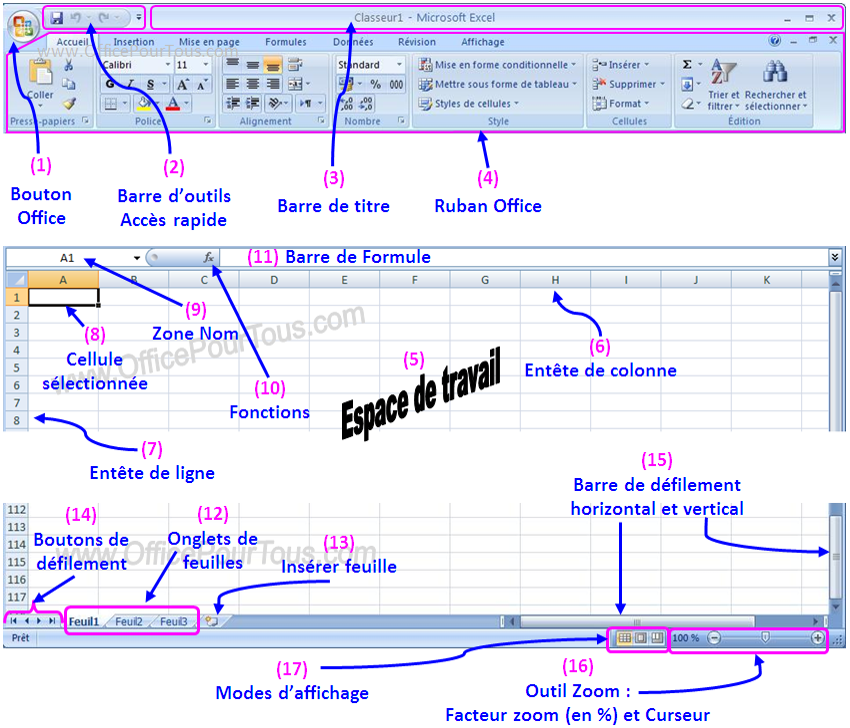
\includegraphics[width=\linewidth]{img/interface}

\begin{definition}[Adressage]
l'adressage est le point de repérage d’une cellule.\\
Une cellule est repéré par deux 2 symboles:  un nombre et une lettre.
\begin{itemize}
	\item La lettre permet de repérer une cellule verticalement.
	\item Le nombre permet de repérer une cellule horizontalement. 
\end{itemize}
\begin{center} 
	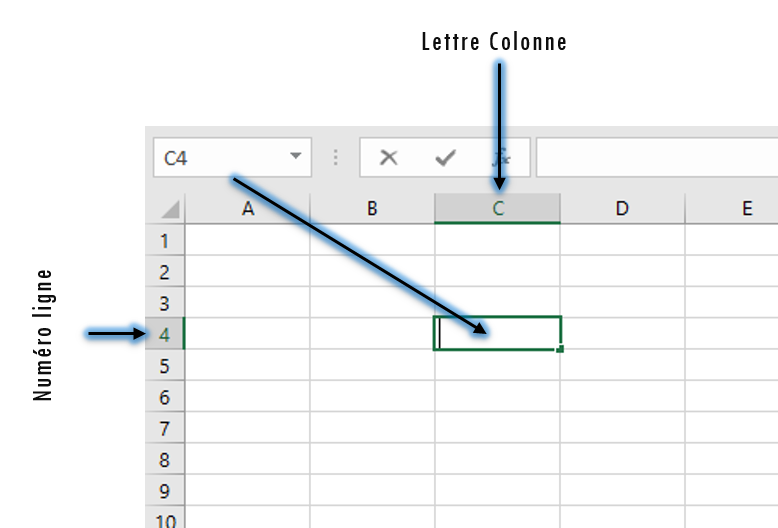
\includegraphics[scale=0.2,width=\linewidth]{img/adressage} 
	\captionof{figure}{Adressage d'une cellule} \label{rdp}
\end{center}
\end{definition}

\begin{definition}[Ruban]
	Il regroupe les fonctionnalités du logiciel, celui-ci évolué  graphiquement avec les mise à jours.\\
	Le ruban est composé d’onglet qui dont de gauche à droite: Accueil, Insertion, Mise en page, formules, Données, Révision, Affichage.
	Ainsi chaque onglet est subdivisé en groupe de même famille.
	\begin{center} 
		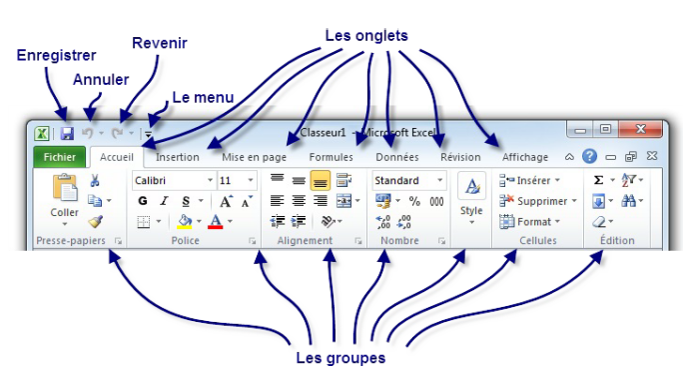
\includegraphics[scale=0.2,width=\linewidth]{img/ruban} 
		\captionof{figure}{Ruban} \label{rdp}
	\end{center}
\end{definition}

	\begin{wrapfigure}{r}{0.2\textwidth}
		\vspace{-2pt}
		\begin{center}
			
\includegraphics[width=0.2\textwidth]{img/barre_access_rapide}
		\end{center}  
		\vspace{-2pt}  
	\end{wrapfigure}
\subsection*{}
\begin{definition}[Barre d'outils Accès rapide]
	
	Comme son nom l’indique, elle permet l'accès rapide aux fonctionnalités globalement utilisées d'Excel.
 
  \textbf{Raccourci clavier: }
 \begin{itemize}
 	\item Ctrl + S: Enregistrer votre document
 	\item Ctrl + C: Copier la cellule sélectionnée
 	\item Ctrl + V: Coller les éléments copier
 	\item Ctrl + S: Couper les éléments sélectionnée
 	\item Ctrl + Z: Annuler la dernière action
 	\item Ctrl + Y: Répéter la dernière action 
 	\item Ctrl + N:  création d'un nouveau fichier
 	\item Ctrl + P: Impression
 	\item Ctrl + O: Ouvrir un fichier existant 	
 \end{itemize}
\end{definition}
\begin{wrapfigure}{r}{0\textwidth}
 
\end{wrapfigure}
\subsection*{}
\begin{definition}[La barre de formules]
	la zone principale de la barre de formule permet d’afficher le contenu d’une cellule sélectionnée. Il peut contenir du texte, nombre, date, fonction ou formule…
	\paragraph{Insérer une fonction:}{le button fx permet d’insérer une fonction dans le calculs}
\end{definition}
\begin{center} 
	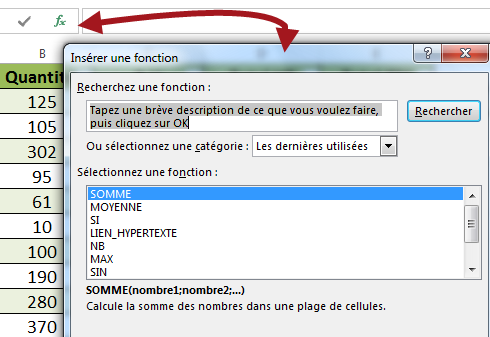
\includegraphics[scale=0.2,width=\linewidth]{img/barre_formule} 
	\captionof{figure}{Barre de Formule} \label{rdp}
\end{center}

\paragraph{Masquer ou afficher la barre de formule}{\hfill\\
 	\begin{enumerate}
 		\item Cliquez sur le menu Fichier => Options.
 		\item Dans la fenêtre qui s’affiche, cliquez sur Options avancées.
 		\item Dans la catégorie Afficher, décochez la case Afficher la barre de formule.
 		\item Validez enfin.
 	\end{enumerate}
 \begin{center} 
 	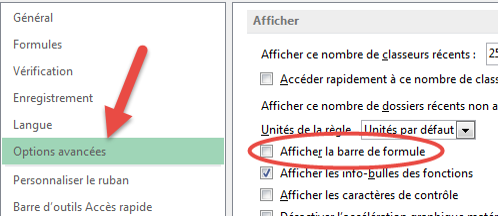
\includegraphics[scale=0.2,width=\linewidth]{img/Masquer_barre} 
 	\captionof{figure}{Masquer ou afficher la barre de formule} \label{rdp}
 \end{center}
}
\paragraph{Empêcher l’affichage des formules dans la barre de formule}{
	Lorsque vous aimez interdire à l’utilisateur de votre classeur Excel de voir les formules utilisées dans une cellule, vous devez faire deux choses :
	\begin{enumerate}
		\item Masquez votre cellule.
			\subitem Pour masquer votre cellule, sélectionnez-la et tapez Ctrl+Mj+\&
			\subitem Choisissez l’onglet Protection et cochez Masquer, puis cliquez sur OK.	
\begin{center} 
	\includegraphics[scale=0.2,width=0.5\linewidth]{img/masquer} 
	\captionof{figure}{Afficher-Masquer formule} \label{rdp}
	\end{center} 
\item Protégez votre feuille.
	\subitem Pour protéger votre feuille, cliquez sur l’onglet Révision puis sur Protéger la feuille.
	\subitem Entrez votre mot de passe et validez.
	\subitem Sélectionnez maintenant votre cellule et remarquez que la barre de formule n’affiche rien.
	
\end{enumerate}
}
\begin{definition}[Barre d'état]

\end{definition}
 \begin{center} 
	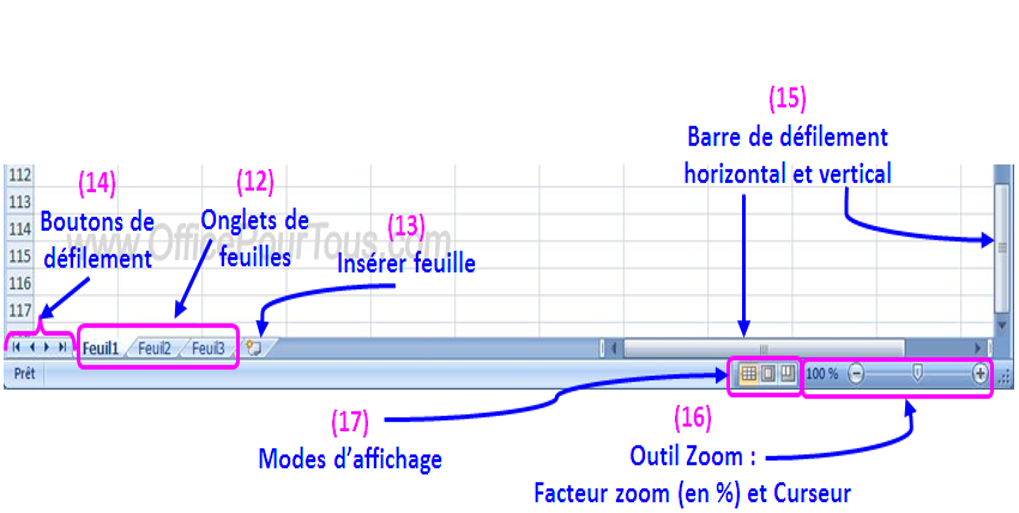
\includegraphics[scale=0.2,width=\linewidth]{img/barre_etat} 
	\captionof{figure}{Barre d'état} \label{rdp}
\end{center}



	\chapter{Premier Classeur}
\section{Création d’un nouveau classeur}
 \begin{center} 
	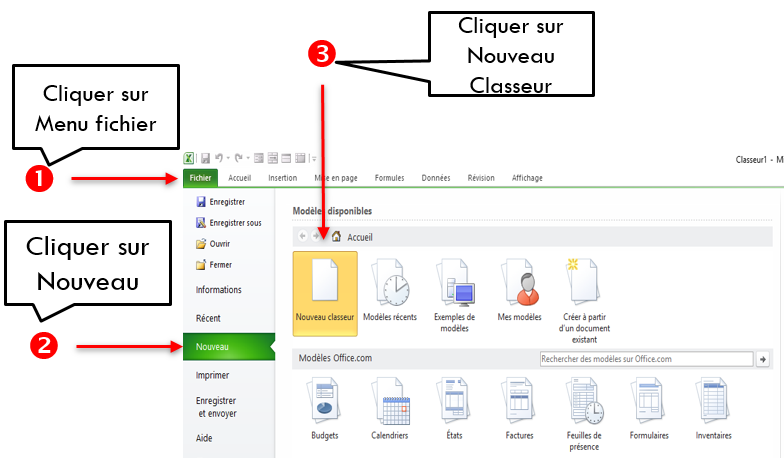
\includegraphics[scale=0.2,width=\linewidth]{img/nouveau_classeur} 
	\captionof{figure}{Création d’un nouveau classeur}
\end{center}
 \begin{center} 
	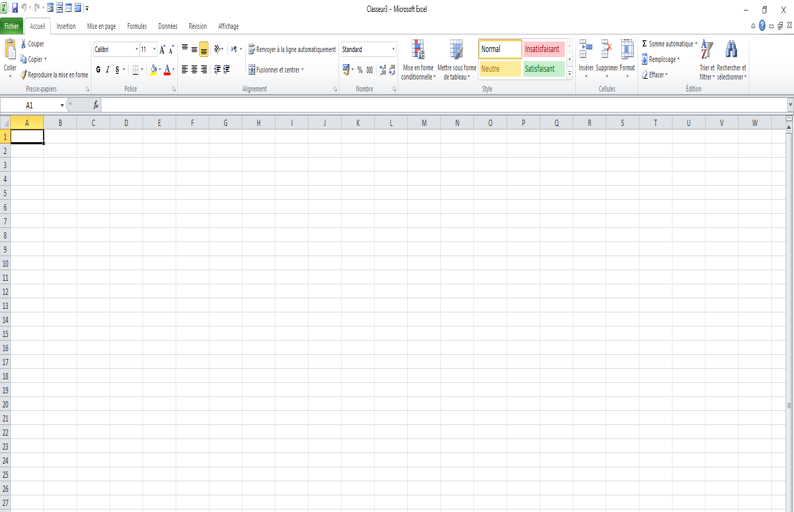
\includegraphics[scale=0.2,width=\linewidth]{img/classeur} 
	\captionof{figure}{Nouveau Classeur}
\end{center}
\section{Enregistrer un classeur la première fois}
\begin{center} 
	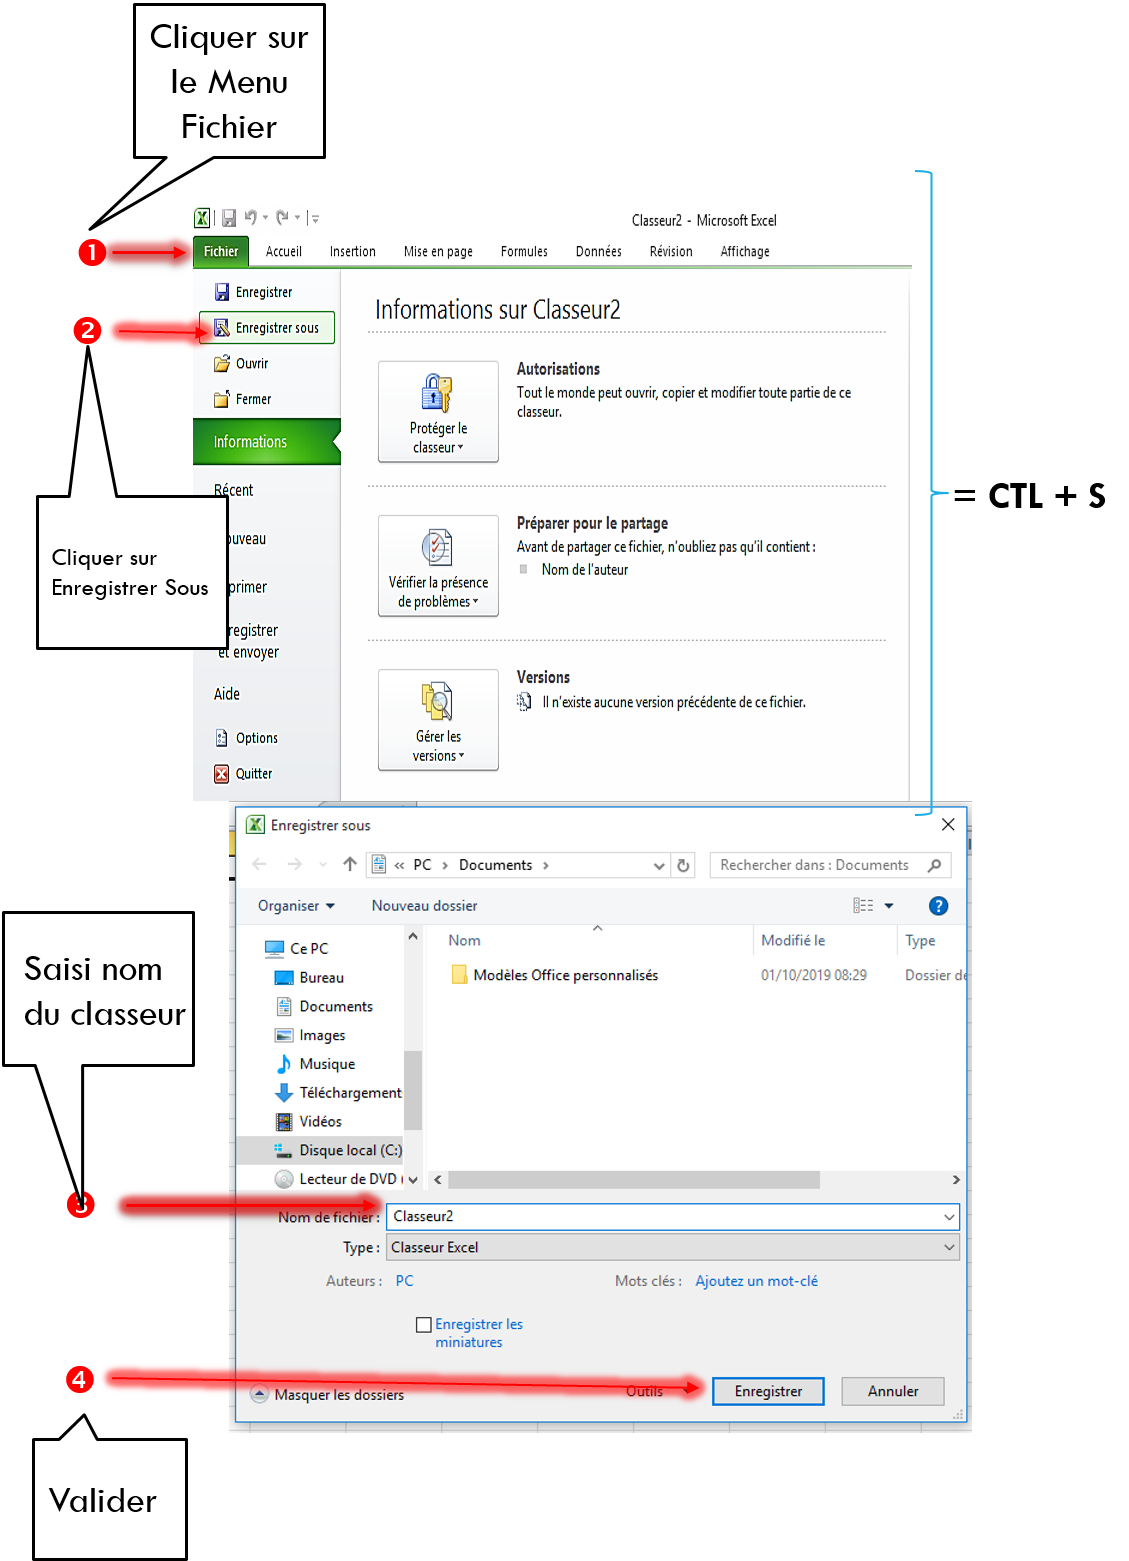
\includegraphics[scale=0.2,width=\linewidth]{img/sauve_as_classeur} 
	\captionof{figure}{Enregistrement d'un classeur la premiere fois} 
\end{center}

\section{Enregistrer les autres fois}
\begin{center} 
	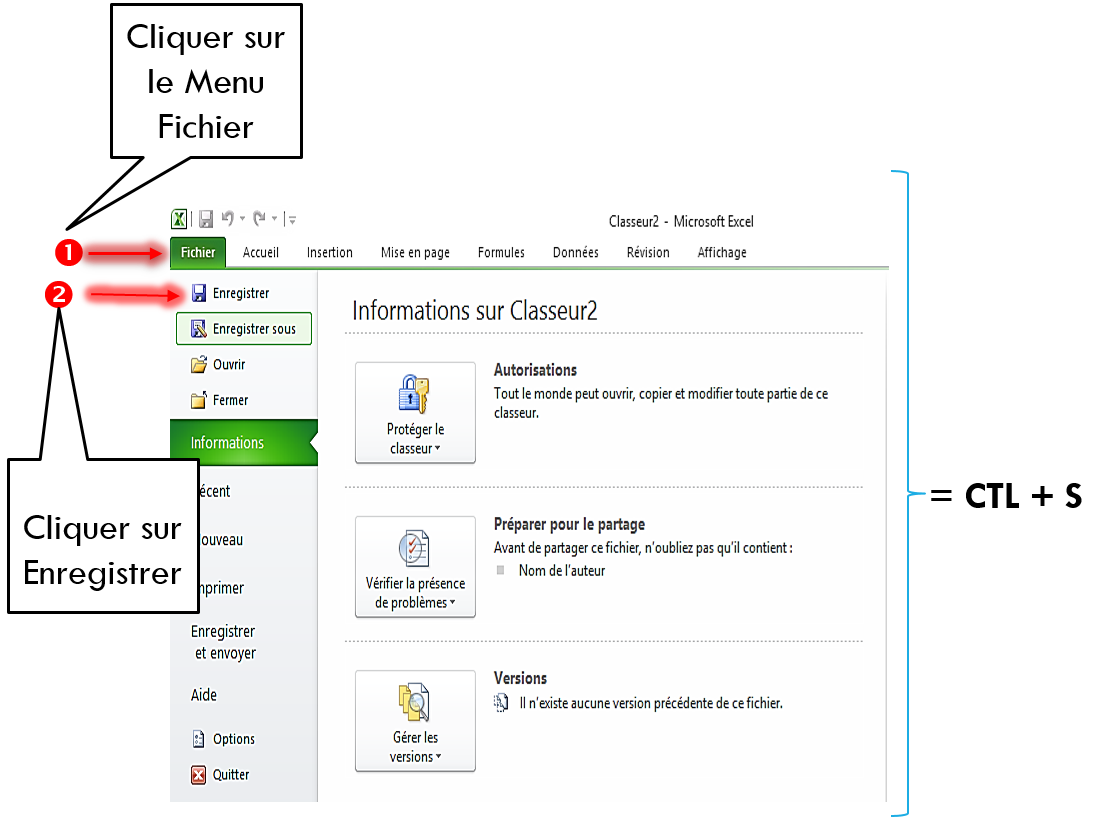
\includegraphics[scale=0.2,width=0.8\linewidth]{img/sauve_classeur} 
	\captionof{figure}{Enregistrement d'un classeur} 
\end{center}
\section{Fermeture d'un classeur}
\begin{center} 
	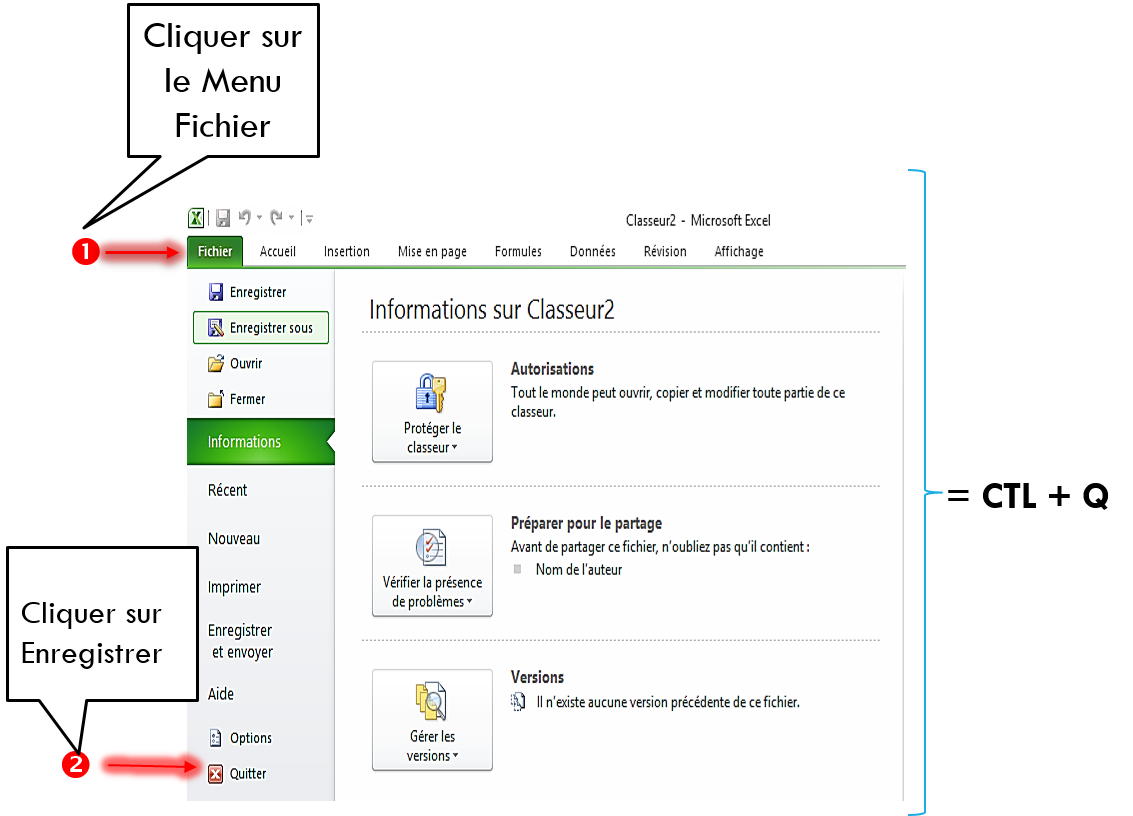
\includegraphics[scale=0.2,width=0.8\linewidth]{img/close_classeur} 
	\captionof{figure}{Fermeture d'un classeur} 
\end{center}

\section{ Saisir du texte et des nombres }
\subsection{ Saisir du texte}
\begin{center} 
	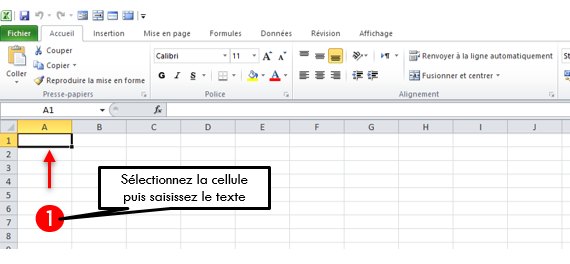
\includegraphics[scale=0.2,width=0.6\linewidth]{img/selecte_cellule} 
 
\end{center}
\begin{center} 
	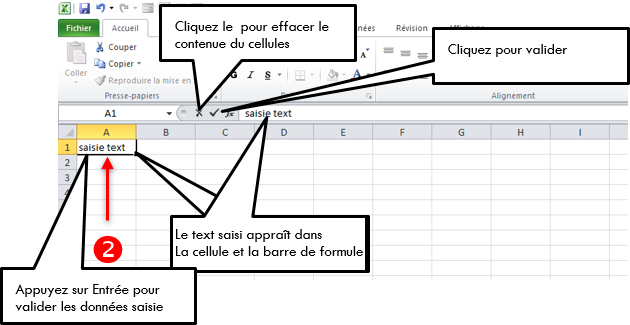
\includegraphics[scale=0.2,width=0.7\linewidth]{img/saisie_text} 
	\captionof{figure}{Saisie du Text} 
\end{center}
\subsection{ Saisir des nombres }
\begin{center} 
	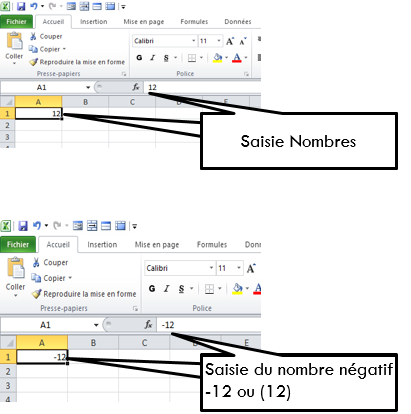
\includegraphics[scale=0.2,width=0.6\linewidth]{img/saisie_nombre} 
	\captionof{figure}{Saisie des nombres} 
\end{center}
\section{Modifier des données} 
\begin{center} 
	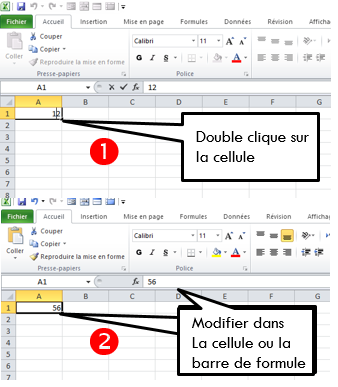
\includegraphics[scale=0.2,width=0.6\linewidth]{img/modification_donner} 
	\captionof{figure}{Modication de donnée} 
\end{center}
\section{Supprimer les données} 
\begin{center} 
	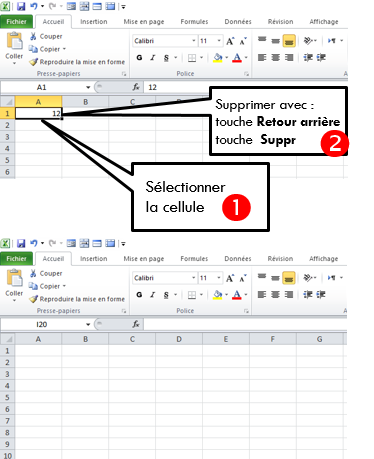
\includegraphics[scale=0.2,width=0.5\linewidth]{img/delete_donner} 
	\captionof{figure}{Supprimer les données} 
\end{center}
\section{Déplacez ou copiez des données} 
	\begin{center} 
		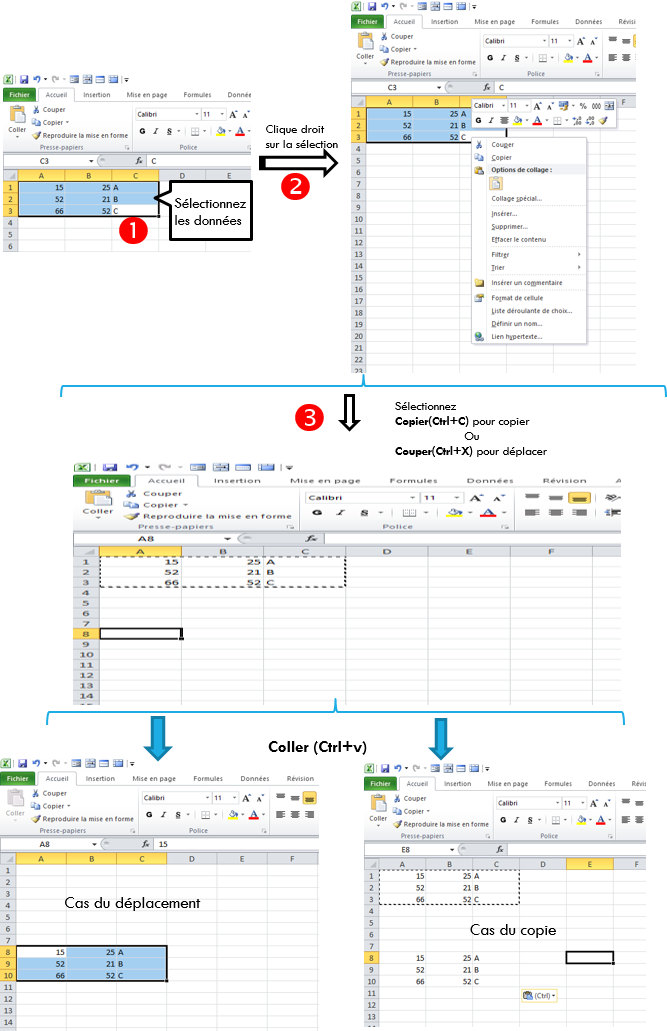
\includegraphics[scale=0.2,width=0.9 \linewidth]{img/deplacer_donner} 
		\captionof{figure}{Supprimer les données} 
	\end{center}
\section{Agrandir les cellules} 
\begin{center} 
	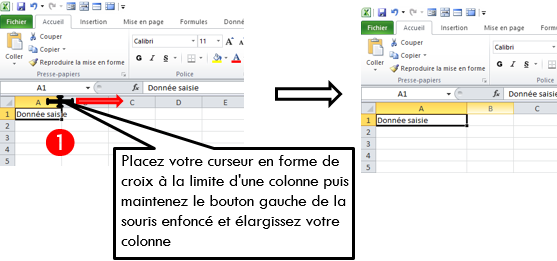
\includegraphics[scale=0.2,width=0.9 \linewidth]{img/agrandir_cellule} 
	\captionof{figure}{Agrandire Cellule} 
\end{center}
\section{Formats,  mise en forme et poignée de recopie incrémentée}
\subsection{Formats}
\begin{center} 
	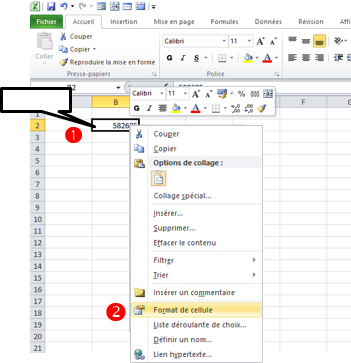
\includegraphics[scale=0.2,width=0.7 \linewidth]{img/format1} 
\end{center}
 \begin{center}  
 	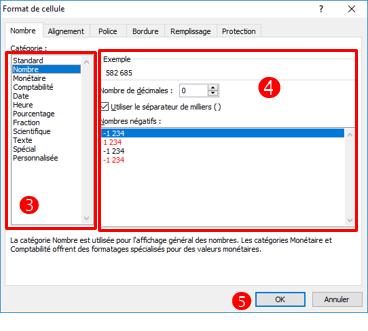
\includegraphics[scale=0.2,width=0.7 \linewidth]{img/format2}
 	\captionof{figure}{Format de donnée} 
 \end{center}
\begin{Exemple}
Cette exemple illustre l'utilisation de formats des nombres
\end{Exemple} 
\begin{center}  
	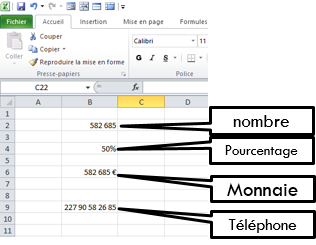
\includegraphics[scale=0.2,width=0.7 \linewidth]{img/exemple_format}
	\captionof{figure}{Exemple Format des nombres} 
\end{center}

\subsection{Mise en forme}
\subsubsection{Bordure}
\begin{center}  
	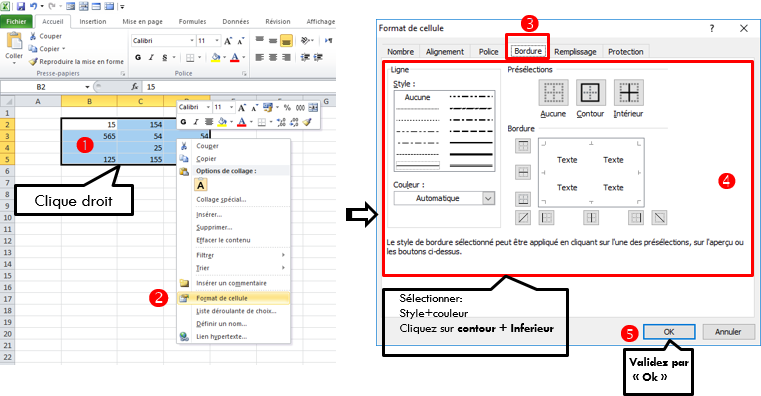
\includegraphics[scale=0.2,width=0.9 \linewidth]{img/bordure_cellule}
		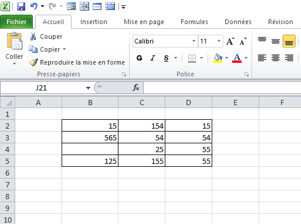
\includegraphics[scale=0.2,width=0.9 \linewidth]{img/tableau_bordure}
	\captionof{figure}{Bordure des cellules} 
\end{center}
\subsubsection{Aligments}
\begin{center}  
	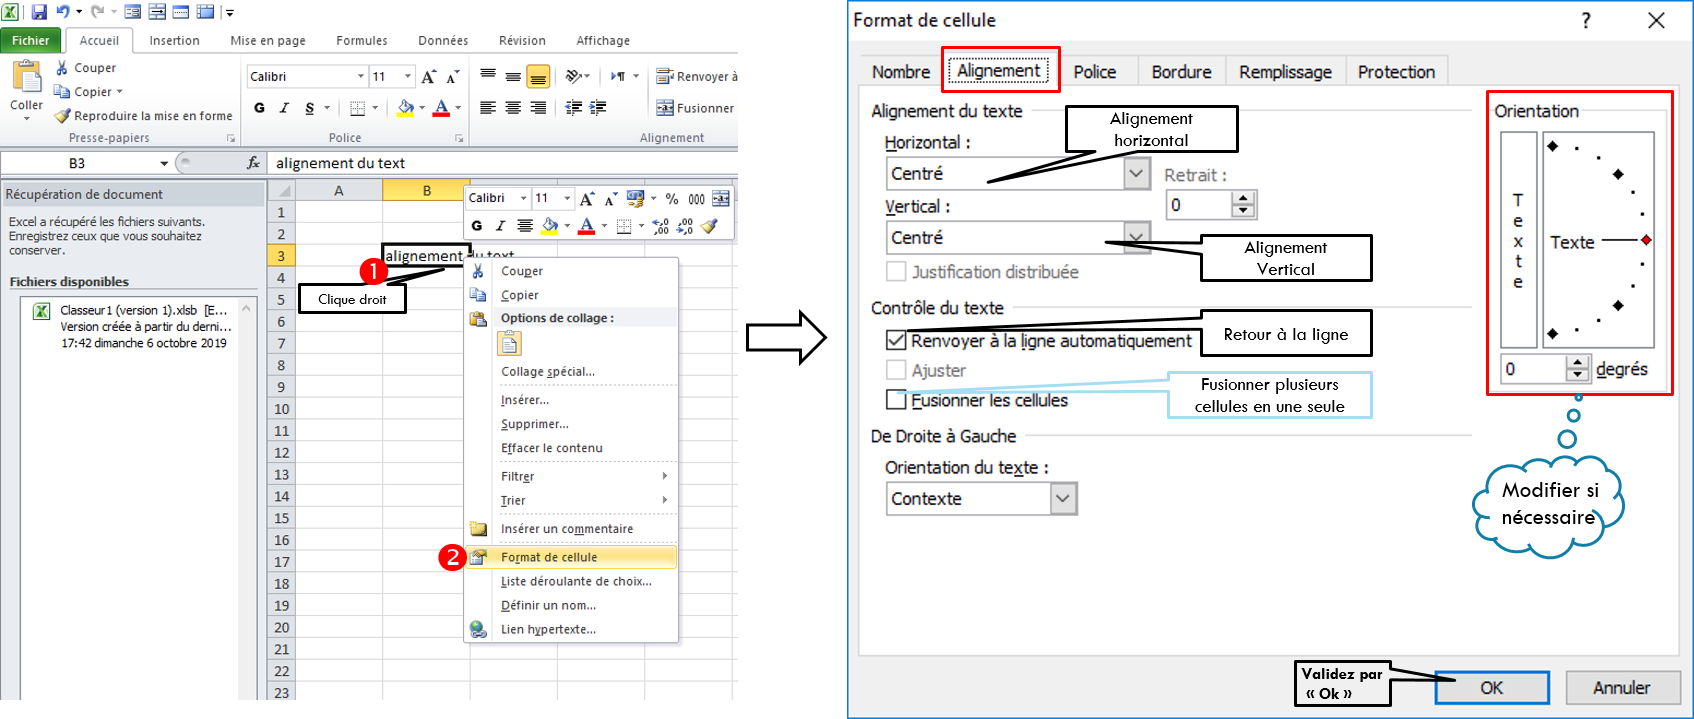
\includegraphics[scale=0.2,width= \linewidth]{img/aligment_text}
	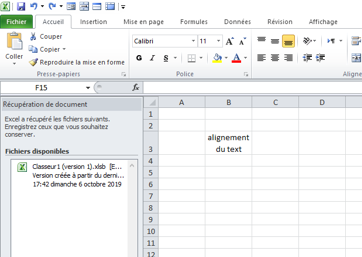
\includegraphics[scale=0.2,width= \linewidth]{img/aligment_exemple}
	\captionof{figure}{Aligment text} 
\end{center}
\subsubsection{Police}
\begin{center}  
	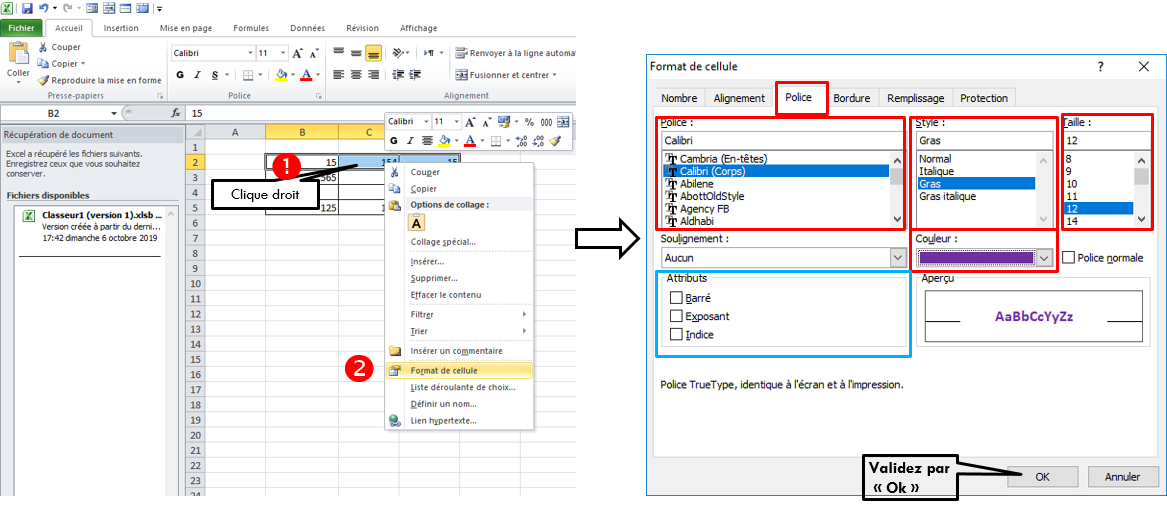
\includegraphics[scale=0.2,width= \linewidth]{img/police_text}
	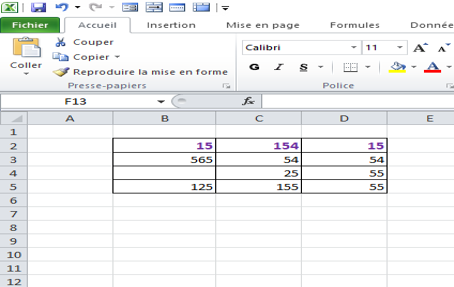
\includegraphics[scale=0.2,width= \linewidth]{img/police_exemple}
	\captionof{figure}{Police text} 
\end{center}
\subsubsection{Trames des Cellules}
\begin{center}  
	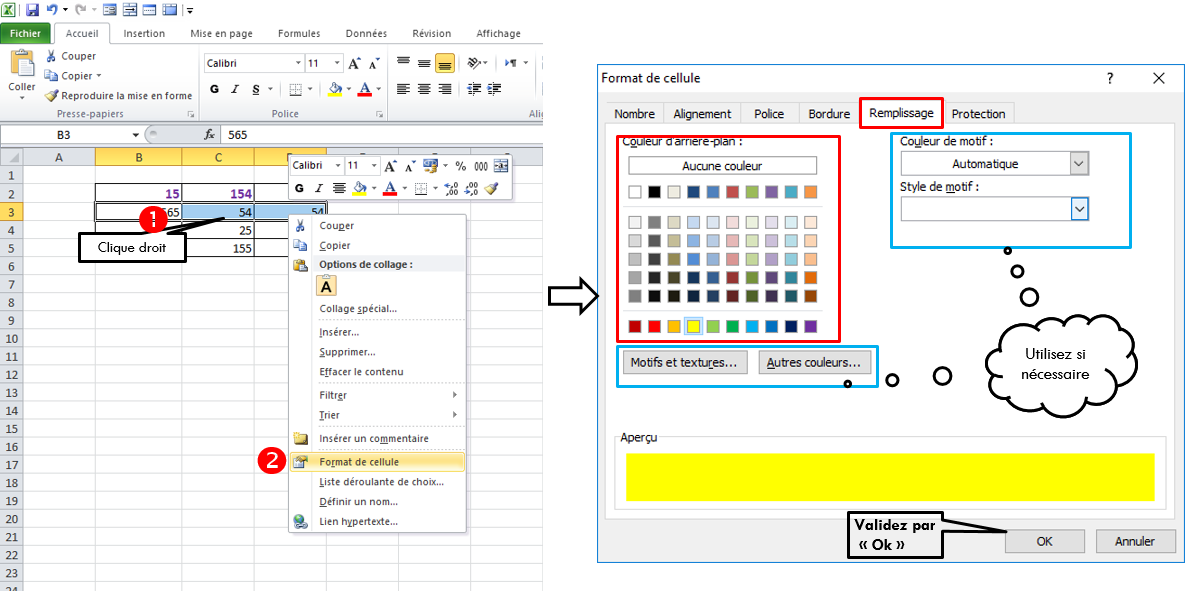
\includegraphics[scale=0.2,width= \linewidth]{img/trame_cellule}
	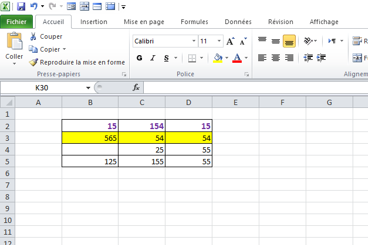
\includegraphics[scale=0.2,width= \linewidth]{img/trame_exemple}
	\captionof{figure}{Trames des cellules} 
\end{center}
\section{Série d'Exercices}
\begin{exercice}\label{ex03}
	Consignes :
\begin{enumerate}
	
	\item  Saisir le tableau.  				
	\item  Mettre la mise en forme le tableau: style titre en gras, taille de police: titre=12, autre=11, police Calibri.				
	\item  Saisir le titre et le centrer horizontalement et veriticalement.				
	\item  Centré les nombres .
\end{enumerate}
\end{exercice} 
\begin{figure}[H]  
	\centering
	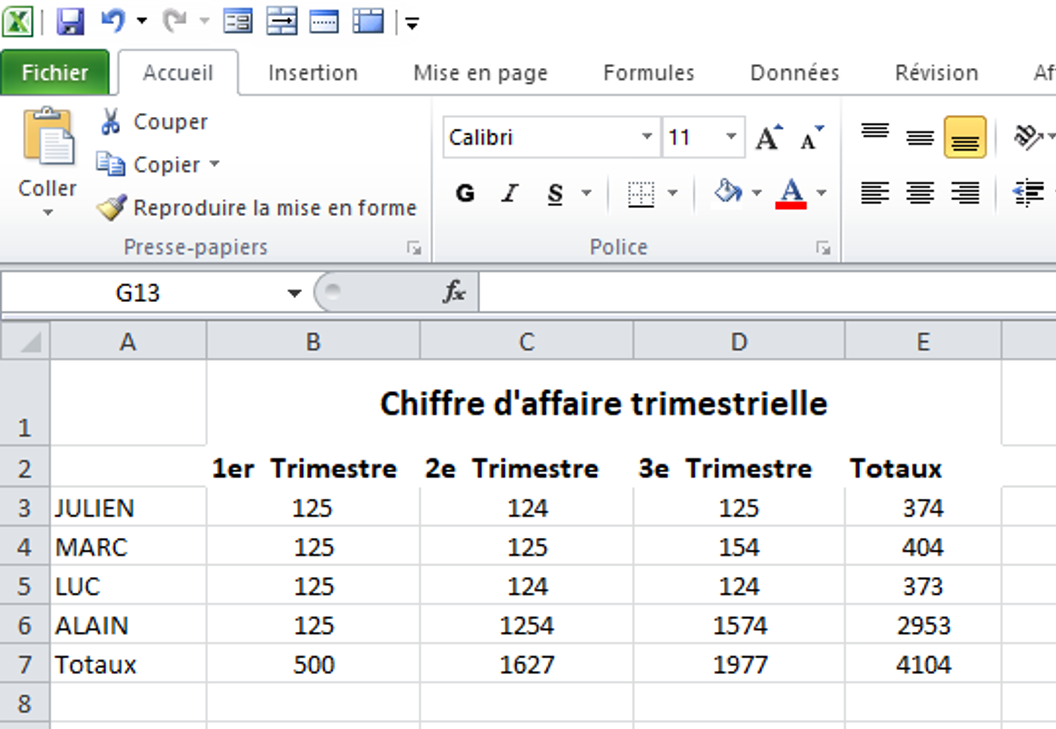
\includegraphics[scale=0.2,width=0.7 \linewidth]{img/ex03} 
	\captionof{figure}{Exercice \ref{ex3}} 
\end{figure} 

\begin{exercice}\label{ex1}
	Consignes :
 	\begin{enumerate}
 				
 	\item  Copier le Tableau de l'exercice \ref{ex03} dans une nouvelle feuille .  				
 	\item  Mettre la mise en forme le tableau: bordures, Trames, style titre en gras, taille de police: titre=12, autre=11, police Calibri.				
 	\item  Saisir le titre et le centrer horizontalement et veriticalement.				
 	\item  Utiliser le format nombre: 3 chiffre apres la virgule ainsi le separateur de mille.				
 		
 	\end{enumerate}
\end{exercice}  
\begin{figure} [H]  
	\centering
	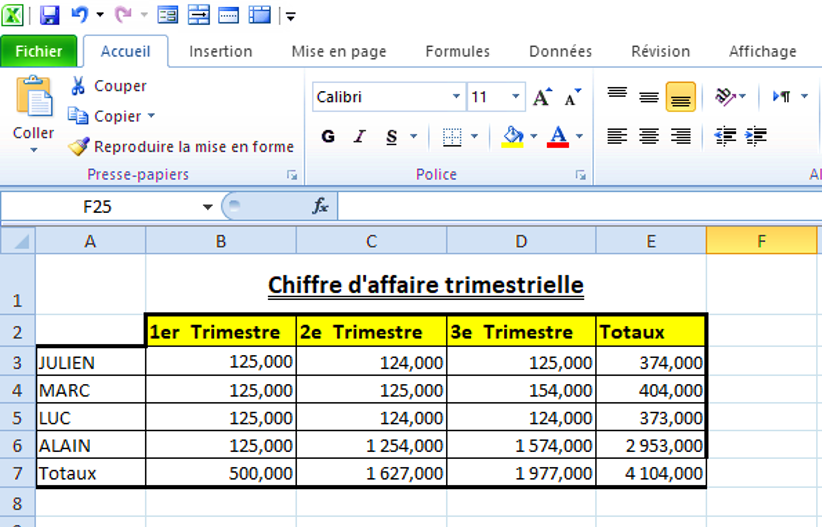
\includegraphics[scale=0.2,width=0.7 \linewidth]{img/ex01} 
	\captionof{figure}{Exercice \ref{ex1}} 
\end{figure}
\begin{exercice}\label{ex2}
	Consignes :
	\begin{enumerate}
		
		\item  Copier le Tableau de l'exercice \ref{ex1} dans une nouvelle feuille.  				
		\item  Mettre la mise en forme le tableau: bordures, Trames, style titre en gras, taille de police: titre=12, autre=11, police Calibri.				
		\item  Saisir le titre et le centrer horizontalement et veriticalement.				
		\item  Utiliser le format nombre: 3 chiffre apres la virgule ainsi le separateur de mille.
	\end{enumerate}	
\end{exercice}
\begin{figure}[H]
	\centering
	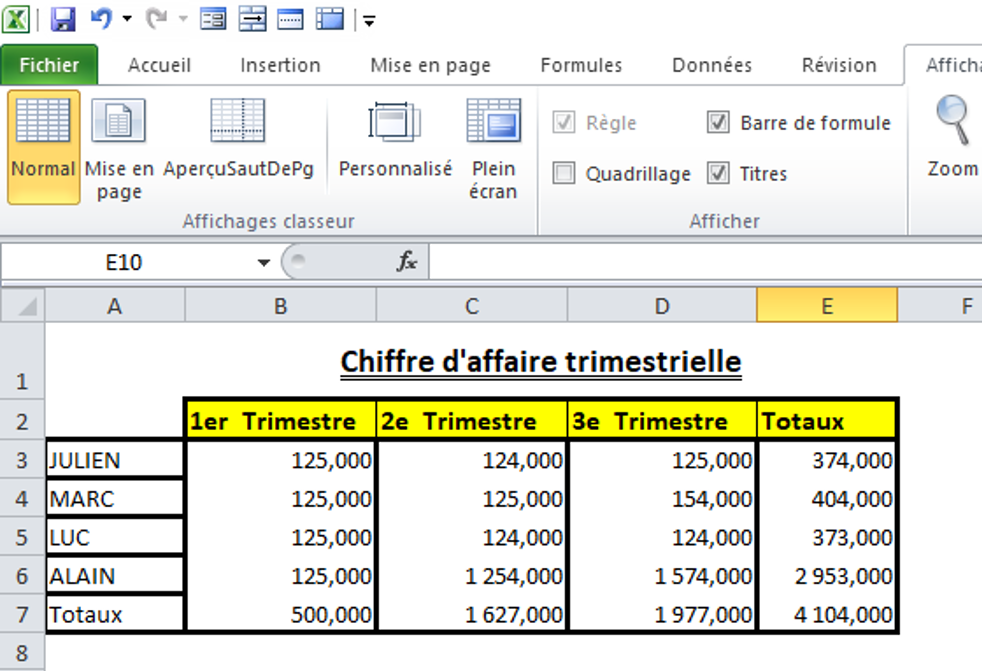
\includegraphics[scale=0.2,width=0.7 \linewidth]{img/ex02} 
	\captionof{figure}{Exercice \ref{ex2}} 
\end{figure}

 
	\chapter{Saisie Rapide}
\section*{}
La recopie incrémentée permet un gain de temps considérable, en vous évitant de répéter maintes fois les mêmes opérations. Pour ce faire, placez le pointeur sur l’extrémité inférieure droite de la sélection, cliquez sans 
relâcher ensuite dirigez le pointeur jusqu'a la cellule de destination.
\section{Succession de Repetition} 
\begin{center}  
	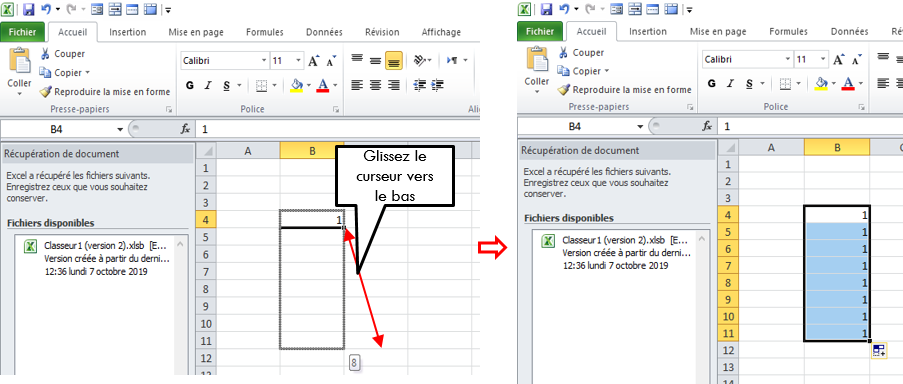
\includegraphics[scale=0.2,width=0.9 \linewidth]{img/saisi_rapide1} 
	\captionof{figure}{Bordure des cellules} 
\end{center}
\section{Suite Inscrementée}
\begin{center}  
	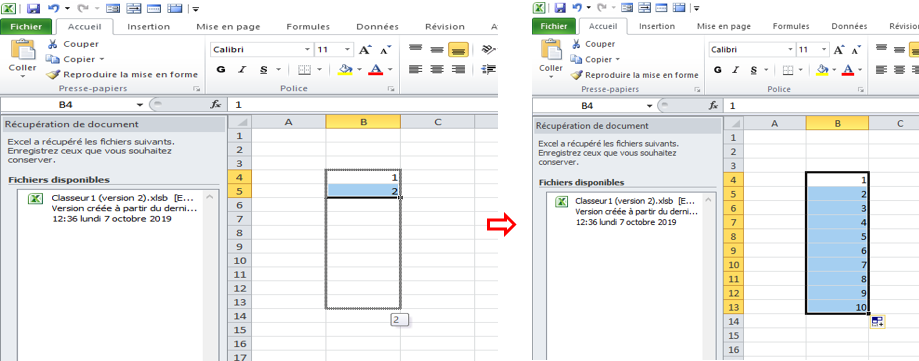
\includegraphics[scale=0.2,width= \linewidth]{img/saisi_rapide2}
	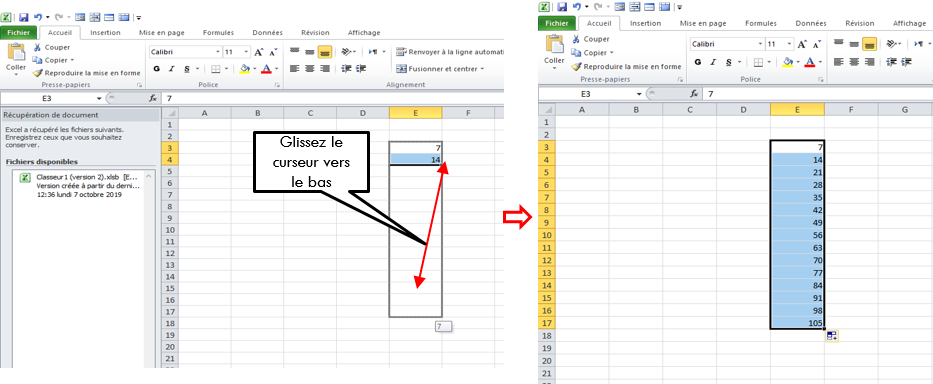
\includegraphics[scale=0.2,width= \linewidth]{img/saisi_rapide3}
	\captionof{figure}{Aligment text} 
\end{center}

\section{Suite Inscrementée  d'une liste personnalisée }
\begin{center}  
	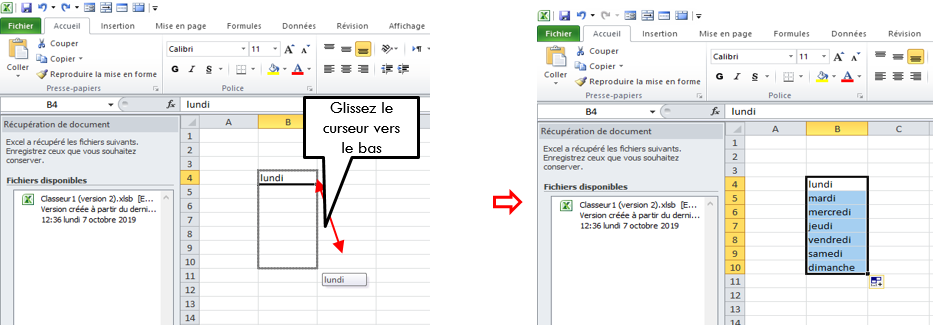
\includegraphics[scale=0.2,width= \linewidth]{img/saisi_rapide4}
	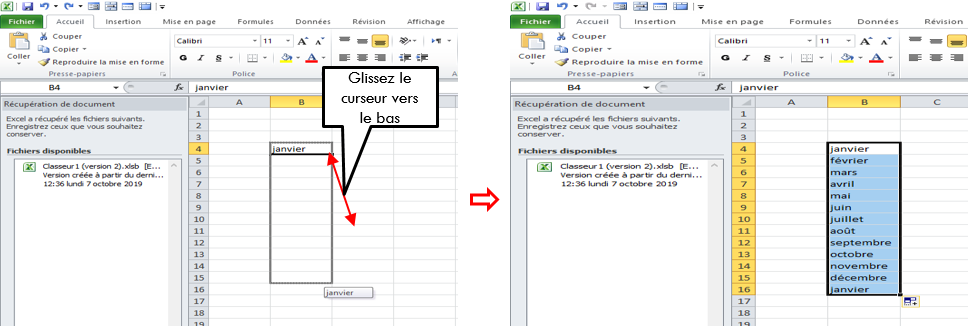
\includegraphics[scale=0.2,width= \linewidth]{img/saisi_rapide5}
	\captionof{figure}{Aligment text} 
\end{center}

\section{Liste personnalisée }
\begin{center}  
	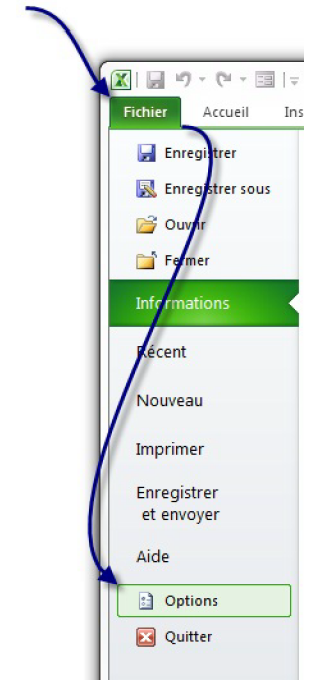
\includegraphics[scale=0.2,width=0.2 \linewidth]{img/saisi_rapide6}
	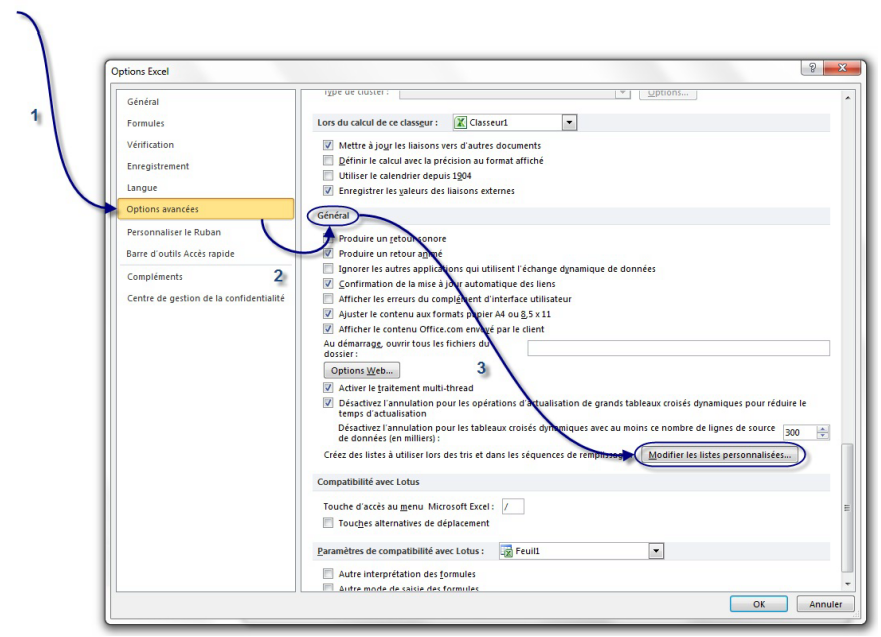
\includegraphics[scale=0.2,width= \linewidth]{img/saisi_rapide7}
	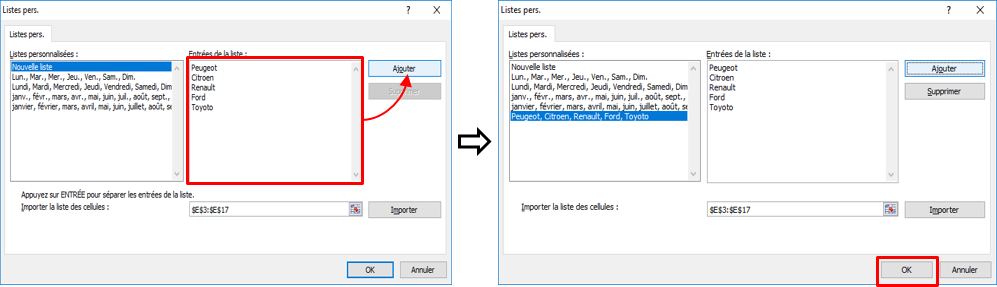
\includegraphics[scale=0.2,width= \linewidth]{img/saisi_rapide8}
	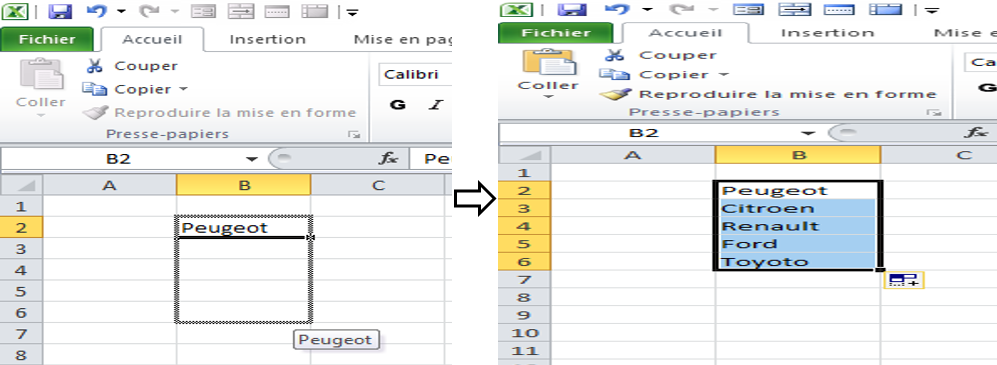
\includegraphics[scale=0.2,width= \linewidth]{img/saisi_rapide9} 
\end{center}

\section{Série d'Exercices}
\begin{exercice}\label{ex4}
	Consignes 
	\begin{enumerate}		
		\item  Saisir  le tableau suivant.
	\end{enumerate}
\end{exercice} 
\begin{figure}[H]  
	\centering
	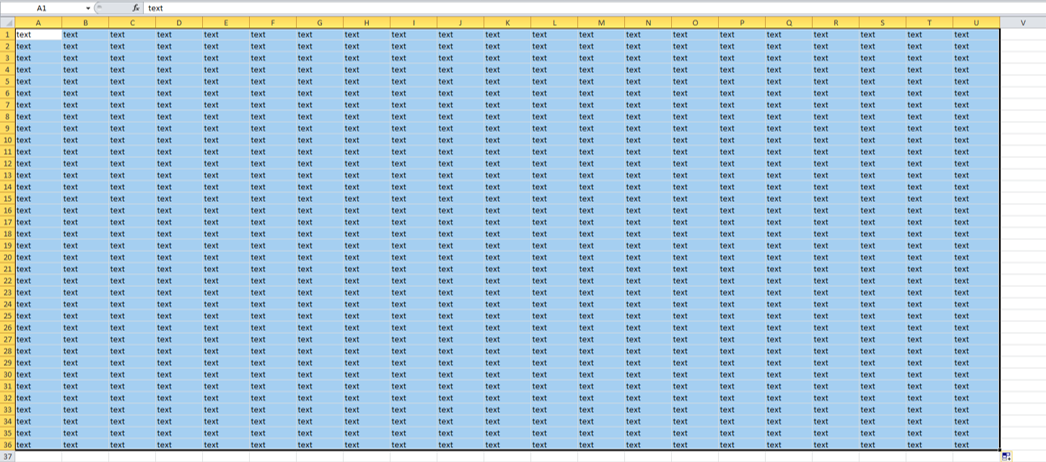
\includegraphics[scale=0.2,width= \linewidth]{img/ex04} 
	\captionof{figure}{Exercice \ref{ex4}} 
\end{figure} 

\begin{exercice}\label{ex5}
	Consignes 
	\begin{enumerate}		
		\item  Saisir  le tableau suivant		
	\end{enumerate}
\end{exercice}  
\begin{figure} [H]  
	\centering
	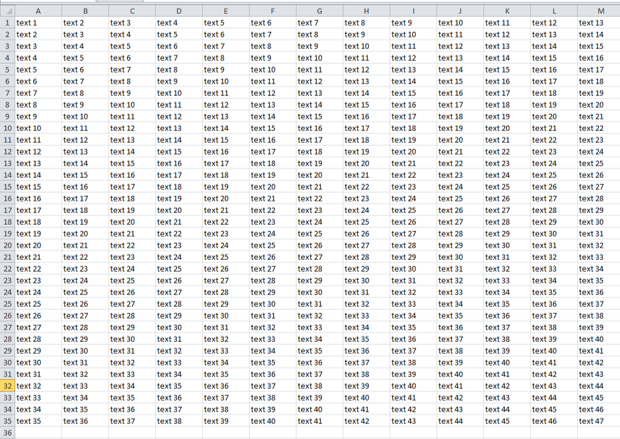
\includegraphics[scale=0.2,width= \linewidth]{img/ex05} 
	\captionof{figure}{Exercice \ref{ex5}} 
\end{figure}
\begin{exercice}\label{ex6}
	Consignes 
	\begin{enumerate}		
		\item  A l'aide du saisie rapide Saisiez le tableau suivant.  				
		\item  Mettre la mise en forme le tableau: largeur colonne:4, centré le contenue du tableau, taille de police:11, police: Calibri.				
		\item  Saisir le titre et le centré horizontalement et veriticalement, police:18, police: Calibri, style:Gras.
	\end{enumerate}	
\end{exercice}
\begin{figure}[H]
	\centering
	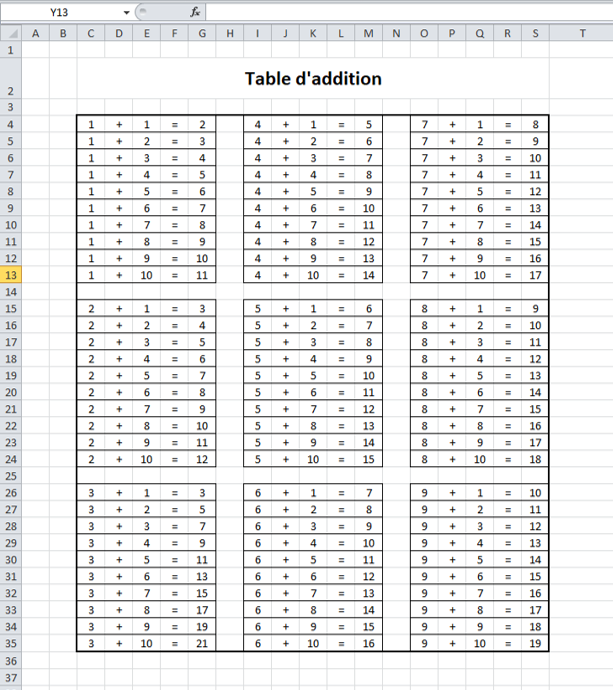
\includegraphics[scale=0.2,width=0.7 \linewidth]{img/ex06}
	\captionof{figure}{Exercice \ref{ex6}} 
\end{figure}

\begin{exercice}\label{ex7}
	Consignes 
	\begin{enumerate}	
		\item Créer une liste personnalisée : \textbf{a,b,c,d,e,f,g,h,i,j,k,l,m,n,o,p,q,r,s,t,u,v,w,x,y,z}
		\item Créer une liste personnalisée : \textbf{z,y,x,w,v,u,t,s,r,q,p,o,n,m,l,k,j,i,h,g,f,e,d,c,b,a}		
		\item  A l'aide du saisie rapide realiser le tableau suivant.  				
		\item  Mettre la mise en forme le tableau:bordure, trame, largeur colonne:4, centré le contenue du tableau, taille de police:11, police: Calibri.
	\end{enumerate}	
\end{exercice}
\begin{figure}[H]
	\centering
	\includegraphics[scale=0.2,width=0.7 \linewidth]{img/ex07}
	\captionof{figure}{Exercice \ref{ex7}} 
\end{figure}

	\chapter{Fonctions}
\section*{}
Excel dispose un ensemble d'outils pour réaliser des calculs de maniere dynamique ou static. La performance de cette logiciel permet de calculer le resultat des milliers de cellules grace à une fonction définie(écrite par l'utilisateur) ou prédéfinie( existe déja).

\begin{center}  
	\includegraphics[scale=0.2,width= \linewidth]{img/fonctions}
	\includegraphics[scale=0.2,width= \linewidth]{img/fonctions2}
\end{center}

\section{Fonctions Arithmétique}
\textbf{{{ Méthode 1}}}
\begin{center}  
	\includegraphics[scale=0.2,width= \linewidth]{img/arithmetique1} 
	\captionof{figure}{Syntaxe d'une formule Arithmétique} 
\end{center}
\begin{Exemple}
\end{Exemple}
\begin{center}  
	\includegraphics[scale=0.2,width= \linewidth]{img/arithmetique2} 
	\captionof{figure}{Operateur Arithmétique } 
\end{center}
\newpage
\textbf{{{ Méthode 2}}}

\begin{center}  
	\includegraphics[scale=0.2,width= \linewidth]{img/arithmetique3} 
\end{center}

\begin{Exemple}
\end{Exemple}
\begin{center}  
	\includegraphics[scale=0.2,width= \linewidth]{img/fonctions3} 
	\captionof{figure}{Operateur Arithmétique fonction prédefinie} 
\end{center}

\section{Série d'Exercices}

\begin{exercice}\label{ex8}
	Consignes 
	\begin{enumerate}		
		\item  Saisissez le tableau  de la Figure (\ref{exo8}) à l'aide du saisie rapide.  				
		\item  Mettez la mise en forme  du tableau.
		\item  Calculez la somme total des valeurs.
	\end{enumerate}	
\end{exercice}
\begin{figure}[H]
	\centering
	\includegraphics[scale=0.2,width= \linewidth]{img/ex08}
	\captionof{figure}{Exercice \ref{ex8}} \label{exo8}
\end{figure}

\begin{exercice}\label{ex9}
	Consignes 
	\begin{enumerate}		
		\item  Saisissez le tableau  de la Figure (\ref{exo9}) à l'aide du saisie rapide.  				
		\item  Mettez la mise en forme  du tableau.
		\item  Calculez le produit total des valeurs.
	\end{enumerate}	
\end{exercice}
\begin{figure}[H]
	\centering
	\includegraphics[scale=0.2,width= \linewidth]{img/ex09}
	\captionof{figure}{Exercice \ref{ex9}} \label{exo9}
\end{figure}

\begin{exercice}\label{ex10}
	Consignes 
	\begin{enumerate}		
		\item  Saisissez le tableau  de la Figure (\ref{exo10}).  				
		\item  Mettez la mise en forme  du tableau.
		\item  Calculez la Somme Note,  tel que Somme Note=Note1 + Note2+Note3.
		\item  Calculez la Moyenne Matière,  tel que Moyen Matière= (Somme Note) / (Nombre de Notes).
		\item  Calculez la Note Matière ,  Note Matière = (Moyen Matière)* Coefficient.
		\item  Calculez la Moyenne,  tel que Moyenne= (Total note Matière)/ (Total Coefficient).
		\subitem NB: Total X= somme des éléments de X
		\item Centrer les valeurs calculées			
	\end{enumerate}	
\end{exercice}
\begin{figure}[H]
	\centering
	\includegraphics[scale=0.2,width= \linewidth]{img/ex010}
	\captionof{figure}{Exercice \ref{ex10}} \label{exo10}
\end{figure}

\section{Autres Fonctions}
\subsection{Fonction de Recherche: minimum \& maximum }
La fonction de recherche (minimum \& maximum) consiste à trouver la valeur minimum(maximum) sur un ensemble de valeurs données, pour se faire
\begin{center}  
	\includegraphics[scale=0.2,width= \linewidth]{img/minimum} 
	\captionof{figure}{Fonction minimum} 
\end{center}

\begin{center}  
	\includegraphics[scale=0.2,width= \linewidth]{img/maximum} 
	\captionof{figure}{Fonction maximum} 
\end{center}

\section{Série d'Exercices}

\begin{exercice}\label{ex11}
	Consignes 
	\begin{enumerate}		
		\item  Saisissez le tableau  de la Figure (\ref{exo11}) à l'aide du saisie rapide.  				
		\item  Mettez la mise en forme  du tableau.
		\item  Calculez le minimum des valeurs du tableau.
	\end{enumerate}	
\end{exercice}
\begin{figure}[H]
	\centering
	\includegraphics[scale=0.2,width= \linewidth]{img/ex011}
	\captionof{figure}{Exercice \ref{ex11}} \label{exo11}
\end{figure}

\begin{exercice}\label{ex12}
	Consignes 
	\begin{enumerate}		
		\item  Saisissez le tableau  de la Figure (\ref{exo12}) à l'aide du saisie rapide.  				
		\item  Mettez la mise en forme  du tableau.
		\item  Calculez le maximum des valeurs du tableau.
	\end{enumerate}	
\end{exercice}
\begin{figure}[H]
	\centering
	\includegraphics[scale=0.2,width= \linewidth]{img/ex012}
	\captionof{figure}{Exercice \ref{ex12}} \label{exo12}
\end{figure}

\begin{exercice}\label{ex13}
	Consignes 
	\begin{enumerate}		
		\item  Saisissez le tableau  de la Figure (\ref{exo13}).  				
		\item  Mettez la mise en forme  du tableau.
		\item  Calculez la Somme Note,  tel que Somme Note=Note1 + Note2+Note3.
		\item  Calculez la Moyenne Matière,  tel que Moyen Matière= (Somme Note) / (Nombre de Notes).
		\item  Calculez la Note Matière ,  Note Matière = (Moyen Matière)* Coefficient.
		\item  Calculez la Moyenne,  tel que Moyenne= (Total note Matière)/ (Total Coefficient).
		\subitem NB: Total X= somme des éléments de X
		\item Calculer le \textbf{maximum1} et \textbf{minimum1} des notes
		\item Calculer le \textbf{maximum2} et \textbf{minimum2} de chaque colonne
		\item Centrer les valeurs calculées			
	\end{enumerate}	
\end{exercice}
\begin{figure}[H]
	\centering
	\includegraphics[scale=0.2,width= \linewidth]{img/ex013}
	\captionof{figure}{Exercice \ref{ex13}} \label{exo13}
\end{figure}


\section{Les conditions}
Les conditions permet de donner des ordres sous certains contrainte. Par exemple si telle cellule vaut \textbf{X}, alors fais \textbf{ceci},	sinon, fais	
  \textbf{cela}	

\subsection{Les Conditions Simples}
\begin{figure}[H]
	\centering
	\includegraphics[scale=0.2,width= \linewidth]{img/conditions_syntaxt}
	\captionof{figure}{Syntaxe d'une condition simple}
\end{figure}

\begin{Exemple}
	Cette exemple illustre l'utilisation des conditions simples
\end{Exemple}
\begin{center}  
	\includegraphics[scale=0.2,width=\linewidth]{img/condition_exemple}
	\captionof{figure}{Exemple condition simple} 
\end{center}

\subsection{Les Conditions Multiples}
Les conditions simples permet de tester que deux (02) valeurs, Il est alors impossible de tester une tranche de valeurs. L'utilisation des operateurs logique permet de remedier à ce problèmes.

\begin{figure}[H]
	\centering
	\includegraphics[scale=0.2,width= \linewidth]{img/condition_multiple}
	\captionof{figure}{Syntaxe condition multiple}
\end{figure}

\begin{Exemple}
	Cette exemple illustre l'utilisation des conditions multiples
\end{Exemple}
\begin{center}  
	\includegraphics[scale=0.2,width=\linewidth]{img/condition_multiple_exemple}
	\captionof{figure}{Exemple condition multiple} 
\end{center}

\section{Série d'Exercices}

\begin{exercice} 
	Consignes 
	\begin{enumerate}		
		\item  Saisissez le tableau  de la Figure (\ref{exo14}).  				
		\item  Mettez la mise en forme  du tableau.
		\item  Le Restants à livrer, tel que Restants à livrer= mod(colonne\_Commande;colonne\_livraison).
		\item  Calculer le total de chaque colonne.
	\end{enumerate}	
\end{exercice}
\begin{center}  
	\includegraphics[scale=0.2,width= \linewidth]{img/ex014} 
	\captionof{figure}{ }\label{exo14}
\end{center}

\begin{exercice} 
	Consignes 
	\begin{enumerate}		
		\item  Saisissez le tableau  de la Figure (\ref{exo15}).  				
		\item  Mettez la mise en forme  du tableau.
		\item Calculez la commission a payé sachant que si la vente depasse 500 alors \textbf{7 Euros} doit etre payée, une fois doublée elle sera donc payée \textbf{14 Euros} sinon \textbf{aucune commission}.
	\end{enumerate}	
\end{exercice}
\begin{center}  
	\includegraphics[scale=0.2,width= \linewidth]{img/ex015} 
	\captionof{figure}{ }\label{exo15}
\end{center}

\begin{exercice} 
	Consignes 
	\begin{enumerate}		
		\item  Saisissez le tableau  de la Figure (\ref{exo15}).  				
		\item  Mettez la mise en forme  du tableau.
		\item Calculez CA TTC.
		\item Calculez Com.
	\end{enumerate}	
\begin{description}
	\item[CA TTC  =]   CA HT  * (1 +  Taux  taxe). 
	\item[Com   =]     CA HT  * (1 +  Taux Com . 
\end{description}
\end{exercice}
\begin{center}  
	\includegraphics[scale=0.2,width= \linewidth]{img/ex016} 
	\captionof{figure}{ }\label{exo15}
\end{center}
\section{Mise en forme conditionnelle}

	\clearpage
 	\part{Contexte de travail}
	\clearpage
	\nopagebreak
 	
 	
\end{document}
